%%%%%%%%%%%%%%%%%%%%%%%%%%%%%%%%%%%%%%%%%%%%%%%%%%%%%%%%%%%%%%%%%%%%%%%%%%%%%%%%
% Towards LLM-Based Affective Perception for Social Robots
% IEEE conference style (IEEEtran, same two-column layout as paperMo/paperMo.tex).
% To use the ieeeconf class instead (as in the Overleaf project), swap the
% \documentclass line for: \documentclass[letterpaper,10pt,conference]{ieeeconf}
% Build: pdflatex -> bibtex -> pdflatex x2
%%%%%%%%%%%%%%%%%%%%%%%%%%%%%%%%%%%%%%%%%%%%%%%%%%%%%%%%%%%%%%%%%%%%%%%%%%%%%%%%

\documentclass[conference]{IEEEtran}
\IEEEoverridecommandlockouts

\usepackage{amsmath}
\usepackage{amssymb}
\usepackage{float}
\usepackage{graphicx}

\graphicspath{{figures/}}

\title{\LARGE \bf
Towards LLM-Based Affective Perception for Social Robots: Evaluating Textual, Visual and Structured Facial Representations}

\author{\IEEEauthorblockN{Thiago Nobre Mascarenhas}
\IEEEauthorblockA{\textit{School of Arts, Sciences and Humanities (EACH)} \\
\textit{University of S\~ao Paulo (USP)}\\
S\~ao Paulo, Brazil}
\and
\IEEEauthorblockN{Monique S. L. S. Tomaz}
\IEEEauthorblockA{\textit{Polytechnic School of Pernambuco (Poli)} \\
\textit{University of Pernambuco (UPE)}\\
Recife, Brazil}
\and
\IEEEauthorblockN{Walter {[Sobrenome]}}
\IEEEauthorblockA{\textit{{[Affiliation to be completed]}} \\
{[City, Country]}}
\and
\IEEEauthorblockN{Wanderson {[Sobrenome]}}
\IEEEauthorblockA{\textit{{[Affiliation to be completed]}} \\
{[City, Country]}}}

\begin{document}

\maketitle
\thispagestyle{empty}
\pagestyle{empty}

\begin{abstract}
Social robots must read human affect from whatever signal is available at a given moment, whether a spoken sentence, a camera frame, or a stream of facial measurements. Large language models (LLMs) are increasingly proposed as the reasoning core of such systems, yet it remains unclear how the form in which affective information is presented to the model shapes what it can perceive. This work asks how three representations of affective information, namely text, native vision, and structured facial features, influence the affective perception of a single multimodal LLM. We evaluate Gemma 4 26B-A4B against task-specific baselines on two complementary benchmarks: continuous valence regression on OMG-Empathy and multi-label Ekman emotion recognition on CMU-MOSEI. The model recognizes emotion from text far better than a trained classifier, reaches parity with a rule-based engine when it sees raw images, and fails badly when facial information is handed to it as serialized numbers. We support these findings with paired non-parametric tests, a Friedman omnibus analysis, bootstrap confidence intervals, and a computational cost report. The advantage of the LLM is therefore not general but tied to the representation, which has direct consequences for how affective perception should be wired into cognitive architectures for human--robot interaction.
\end{abstract}

\bigskip
\noindent\textbf{Keywords:}
Large Language Models, Affective Computing, Multimodal Perception, Emotion Recognition, Human--Robot Interaction, Social Robotics.

\section{Introduction}
Emotion is central to how people perceive situations, make decisions, and coordinate with one another, and the same is increasingly expected of artificial agents that share our spaces~\cite{Picard1997AffectiveComputing, Calvo2010AffectDetection}. For a social robot, reading the affective state of a partner is not a peripheral feature but a prerequisite for behaving in a way that people accept as natural~\cite{Breazeal2003SociableRobots, Fong2003SociallyInteractive}. Decades of work in human--robot interaction (HRI) have established that this perception must operate over several behavioral channels, including facial expression, speech, and prosody, often under noisy and uncontrolled conditions~\cite{Goodrich2007HRISurvey, Spitale2024AffectiveRobotics}.

Large language models have recently entered this picture. Beyond dialogue, they are being used as the reasoning core of robotic systems, translating high-level instructions into action~\cite{Ahn2022SayCan, Zitkovich2023RT2, Kawaharazuka2024RobotLLMSurvey, Vemprala2023ChatGPTRobotics} and, more recently, as affective modules that let a robot ground its responses in the emotional state of its partner~\cite{Magalhaes2024Nadine, Churamani2024EmpathicGrounding, Laban2024LLMsHRI}. The appeal is clear: a model pre-trained on a large corpus carries broad world knowledge and can be queried without task-specific training. What is far less clear is whether this knowledge transfers equally well across the different forms in which affective evidence reaches a robot.

This question matters because affective information does not arrive in a single format. A transcript of what a person said is text. A camera frame is an image. A facial tracker produces a vector of numerical activations. These are three genuinely different representations of the same underlying affect, and an LLM does not necessarily treat them alike. Surveys of affective computing with LLMs report strong results on textual input but a much less settled picture for non-textual signals~\cite{Survey2024AffectiveLLM, Survey2025MLLMEmotion, Survey2024TextCentric}, and recent analyses warn that fluent emotional language does not guarantee fine-grained perceptual accuracy~\cite{Zhang2025FluentUnfeeling}.

We therefore study a single research question: \emph{how do different representations of affective information --- text, vision, and structured features --- influence the performance of LLMs in affective perception tasks?} To answer it, we hold the model fixed (Gemma 4 26B-A4B, a quantized mixture-of-experts model served locally) and vary only the representation given to it, comparing each against a baseline designed for that signal. We evaluate on two complementary datasets, one demanding continuous valence regression from video (OMG-Empathy) and one demanding multi-label emotion classification from pre-extracted features (CMU-MOSEI).

The contribution of this paper is threefold. First, we provide a controlled, modality-by-modality comparison of an LLM against traditional baselines on two affective tasks, with paired statistical testing and effect sizes. Second, we report computational cost and inference latency, an aspect frequently overlooked but decisive for any robotic deployment. Third, we draw out the implications for cognitive architectures in HRI, arguing for a hybrid design in which the representation, not a blanket preference for LLMs, dictates which component should perceive affect.

The remainder of the paper is organized as follows. Section~\ref{sec:background} reviews affective perception, facial representations, and multimodal LLMs. Section~\ref{sec:method} describes the model, datasets, input conditions, baselines, and evaluation protocol. Section~\ref{sec:results} presents the results and their statistical analysis. Section~\ref{sec:discussion} discusses why text and vision succeed while structured features fail, and what this means for social robotics. Section~\ref{sec:cost} reports the computational cost. Sections~\ref{sec:limitations} and~\ref{sec:conclusion} close with limitations and conclusions.

\section{Background}
\label{sec:background}
Affective computing studies how machines can recognize, interpret, and express emotion, and it has long been framed as a multimodal problem in which facial, vocal, and linguistic signals evolve together over time~\cite{Picard1997AffectiveComputing, Calvo2010AffectDetection}. Two views of emotion recur in this literature. The categorical view, rooted in Ekman's basic emotions, assigns discrete labels such as anger or surprise~\cite{Ekman1992BasicEmotions}. The dimensional view, following Russell's circumplex model, places affect on continuous axes of valence and arousal~\cite{Russell1980Circumplex}. Both appear in this work: OMG-Empathy is annotated dimensionally, while CMU-MOSEI is annotated with Ekman intensities.

Among observable signals, the face is the most studied. Supervised deep models now dominate facial expression recognition and define the state of the art on standard benchmarks~\cite{Li2022DeepFER}. A complementary line of work represents the face parametrically through blendshape coefficients, compact descriptors of localized facial deformations that can be estimated in real time from a single camera~\cite{Surdulescu2023Blendshapes}. Such parametric descriptors are attractive for robotics because they are cheap to compute and easy to interpret, and they form the basis of recent affective pipelines for HRI that map facial activity onto a valence--arousal space~\cite{Spitale2024AffectiveRobotics}.

In parallel, multimodal LLMs have made it possible to query a single model with text or images and obtain structured answers without task-specific training. Within robotics, this has driven systems that use the model as a planner or controller~\cite{Ahn2022SayCan, Zitkovich2023RT2, Kawaharazuka2024RobotLLMSurvey} and, increasingly, as an affective component that reasons over a partner's emotional state to shape verbal and non-verbal behavior~\cite{Magalhaes2024Nadine, Churamani2024EmpathicGrounding}. Critical reviews of this trend stress both its promise and its risks, from latency and hallucination to the difficulty of handling ambiguous affect~\cite{Laban2024LLMsHRI}.

A recurring but rarely isolated issue is representation. Transformer tokenizers fragment multi-digit numbers, which destroys the magnitude relationships that traditional classifiers exploit directly on floating-point vectors. Text-centric surveys of multimodal sentiment analysis note that LLMs excel when the signal is linguistic but struggle to ingest dense numerical features serialized as strings~\cite{Survey2024TextCentric, Survey2025MLLMEmotion}. This observation motivates our central comparison: rather than asking whether an LLM is good at affect, we ask which representation of affect it can actually use.

\section{Experimental Setup}
\label{sec:method}
We evaluate a single multimodal LLM, Gemma 4 26B-A4B-it~\cite{Gemma3Team2025, Gemma4Card2026}, a mixture-of-experts (MoE) model with 25.2 billion total parameters and 3.8 billion active per token, quantized to 4-bit integers via AWQ~\cite{Lin2024AWQ}. The model is served through vLLM~\cite{Kwon2023vLLM} on a single NVIDIA L4 24~GB GPU, exposing an OpenAI-compatible API. Inference is orchestrated with LangGraph~\cite{LangGraph2024}, using greedy decoding (temperature~$=0$, maximum 512 output tokens) and manual JSON parsing with schema validation. Holding the model fixed lets us attribute any difference in performance to the input representation rather than to the model or its decoding.

\subsection{Datasets}
OMG-Empathy~\cite{Barros2019OMGEmpathy} provides 80 videos of dyadic interactions (about 7~hours) in which a listener reacts to emotional stories told by an actor. After each session, the listener continuously annotated their affective state on a valence scale from $-1$ to $+1$ using a joystick. We use the official test split (stories 3, 6, and 7; 15 videos from 10 subjects) and follow the challenge protocol, computing the Concordance Correlation Coefficient (CCC)~\cite{Lin1989CCC} per video time series.

CMU-MOSEI~\cite{Zadeh2018MOSEI} contains roughly 23{,}000 annotated segments from YouTube videos, each labeled with intensities for the six basic Ekman emotions~\cite{Ekman1992BasicEmotions}. Because the dataset distributes pre-extracted features rather than raw video, we access it through the CMU Multimodal SDK format~\cite{Zadeh2018MultiAttention}: verbatim transcripts and 35-dimensional FACET visual features~\cite{FACET}. We evaluate on 400 test segments using multi-label F1 (micro, macro, and weighted), treating an emotion as present when its annotated intensity exceeds zero.

\subsection{Input Conditions}
We define three input conditions that vary the modality of the affective signal presented to the model, summarized in Table~\ref{tab:conditions}.

\begin{table}[htbp]
\caption{LLM input conditions by modality and dataset.}
\label{tab:conditions}
\centering
\setlength{\tabcolsep}{4pt}
\renewcommand{\arraystretch}{1.15}
\small
\begin{tabular}{l p{3.6cm} l}
\hline
\textbf{Condition} & \textbf{Input to the LLM} & \textbf{Available in} \\
\hline
\textbf{C1 --- Text} & Verbatim speaker transcript & MOSEI only \\
\textbf{C2 --- Features} & Serialized blendshape statistics (OMG) or FACET coefficients (MOSEI) & Both \\
\textbf{C3 --- Vision} & Three JPEG keyframes per 4\,s window, base64-encoded & OMG only \\
\hline
\end{tabular}
\end{table}

For OMG, facial features are extracted with the MediaPipe Face Landmarker~\cite{Surdulescu2023Blendshapes}: eight frames are sampled uniformly within each 4\,s window, and the 15 most active of the 52 blendshape coefficients are aggregated into their mean, maximum, and standard deviation. The same blendshapes feed both the LLM (condition C2) and the rule-based baseline, which makes that comparison exact. For MOSEI, FACET features are averaged over each segment interval. Condition C3 applies only to OMG, the sole dataset that ships raw video. Both zero-shot and few-shot (in-context) variants are evaluated, with few-shot examples drawn exclusively from the training split to avoid leakage.

\subsection{Baselines}
For OMG-Empathy, the baseline is a rule-based engine that maps the 52 blendshape coefficients to valence and arousal using hand-defined rules grounded in the circumplex model~\cite{Russell1980Circumplex}, with multi-frame aggregation (mean and peak) to match the LLM's temporal window. For CMU-MOSEI, the baseline is a multi-output logistic regression trained on 6{,}000 FACET segments, predicting six independent binary emotion labels; we also report a random-chance baseline (class-proportional sampling) and a majority baseline (always predicting \emph{happiness}). Because the LLM produces conservative integer intensity scores, its emotion threshold is selected by a grid search over $[0.01, 0.50]$ (best value $0.15$ across conditions).

\section{Results}
\label{sec:results}

\subsection{OMG-Empathy: Continuous Valence Regression}
Table~\ref{tab:omg_ccc} reports the mean CCC across the 15 test videos, with bootstrap 95\% confidence intervals (10{,}000 resamples) and inter-video standard deviations. Figure~\ref{fig:omg_conditions} shows the same values graphically.

\begin{table}[htbp]
\caption{Mean CCC ($\pm$ SD) and 95\% bootstrap CI for OMG-Empathy ($n=15$ videos).}
\label{tab:omg_ccc}
\centering
\setlength{\tabcolsep}{4pt}
\renewcommand{\arraystretch}{1.15}
\small
\begin{tabular}{l c c c}
\hline
\textbf{System} & \textbf{Mean CCC} & \textbf{95\% CI} & \textbf{SD} \\
\hline
LLM C3 (vision), zero-shot & \textbf{+0.158} & [+0.085, +0.230] & 0.146 \\
Baseline (rules, multi-frame) & +0.148 & [+0.044, +0.259] & 0.212 \\
LLM C2 (blendshapes), $k=3$ & +0.127 & [+0.046, +0.213] & 0.165 \\
LLM C2 (blendshapes), 0-shot & +0.090 & [+0.007, +0.176] & 0.166 \\
\hline
\end{tabular}
\end{table}

\begin{figure}[!ht]
\centering
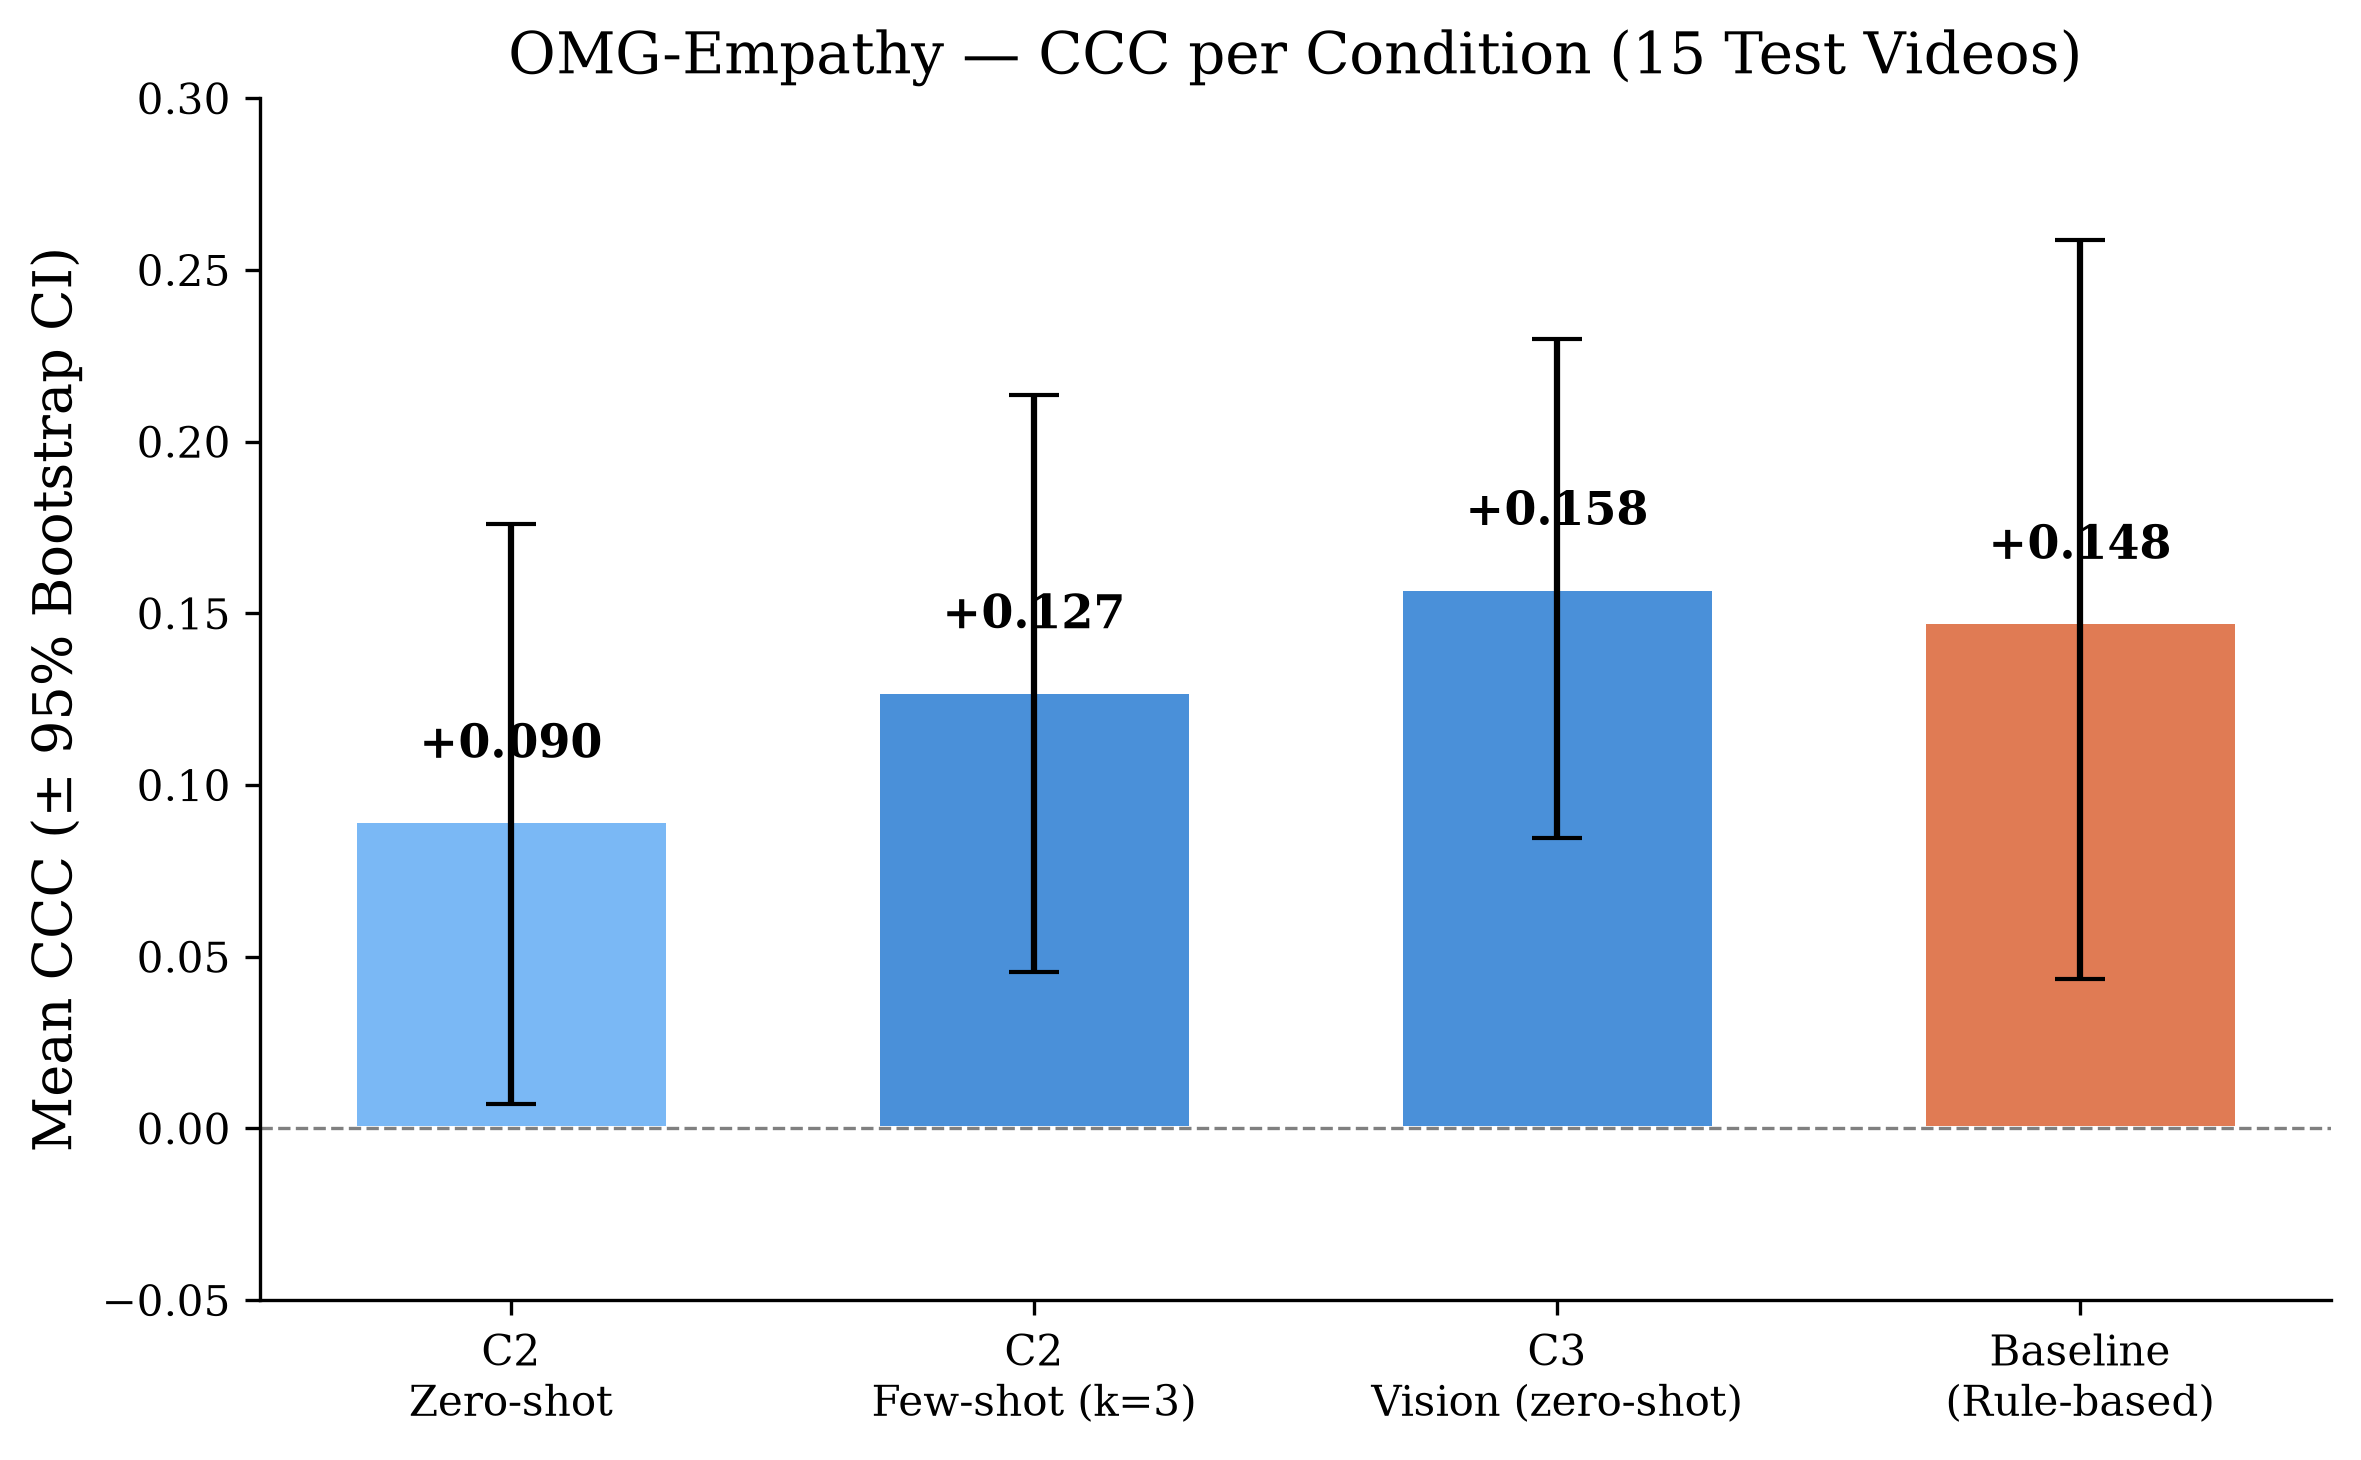
\includegraphics[width=0.46\textwidth]{omg_ccc_conditions.png}
\caption{Mean CCC per condition with 95\% bootstrap confidence intervals on OMG-Empathy. Native vision (C3) is statistically indistinguishable from the rule-based baseline.}
\label{fig:omg_conditions}
\end{figure}

With native vision (C3), the model reaches a CCC of $+0.158$, slightly above the rule-based baseline at $+0.148$. The difference is not significant: a Wilcoxon signed-rank test~\cite{Wilcoxon1945} gives $W=45.0$, $p=0.421$, with a negligible effect size ($d=+0.07$, following Cohen~\cite{Cohen1988}), and the bootstrap intervals~\cite{Efron1993Bootstrap} overlap heavily. The only significant pairwise difference is between the baseline and C2 in the zero-shot setting ($W=17.0$, $p=0.013$, $d=+0.64$), where the model is clearly worse once facial information is serialized as numbers. Table~\ref{tab:omg_wilcoxon} lists all pairwise tests.

\begin{table}[htbp]
\caption{Pairwise Wilcoxon signed-rank tests between conditions ($n=15$ videos).}
\label{tab:omg_wilcoxon}
\centering
\setlength{\tabcolsep}{4pt}
\renewcommand{\arraystretch}{1.15}
\small
\begin{tabular}{l c c c c}
\hline
\textbf{Comparison} & \boldmath$\Delta$ & \textbf{W} & \textbf{p} & \boldmath$d$ \\
\hline
C3 vs.\ Baseline & +0.010 & 45.0 & 0.421 & +0.07 \\
C3 vs.\ C2 (0-shot) & +0.068 & 30.0 & 0.095 & +0.57 \\
C2 ($k{=}3$) vs.\ C2 (0-shot) & +0.038 & 32.0 & 0.121 & +0.51 \\
C2 ($k{=}3$) vs.\ Baseline & $-0.020$ & 38.0 & 0.229 & $-0.30$ \\
Baseline vs.\ C2 (0-shot) & +0.058 & 17.0 & \textbf{0.013} & +0.64 \\
\hline
\end{tabular}
\end{table}

To test for a global difference among the four conditions, we applied a Friedman test~\cite{Friedman1937} --- the non-parametric counterpart of a repeated-measures ANOVA, appropriate here because the per-video CCCs are non-normally distributed and the sample is small ($n=15$). The result is significant ($\chi^2 = 10.04$, $p=0.018$, Kendall's $W=0.223$), indicating that at least one condition differs from the others. Mean ranks order the conditions as native vision (1.87), baseline (2.13), C2 few-shot (2.80), and C2 zero-shot (3.20), where a lower rank is better. However, after Holm--Bonferroni correction no single pairwise comparison remains significant, the closest being baseline versus C2 zero-shot (adjusted $p=0.075$). The omnibus signal is thus real but diffuse, consistent with the high inter-video variance shown in Figure~\ref{fig:omg_per_video}.

\begin{figure*}[!ht]
\centering
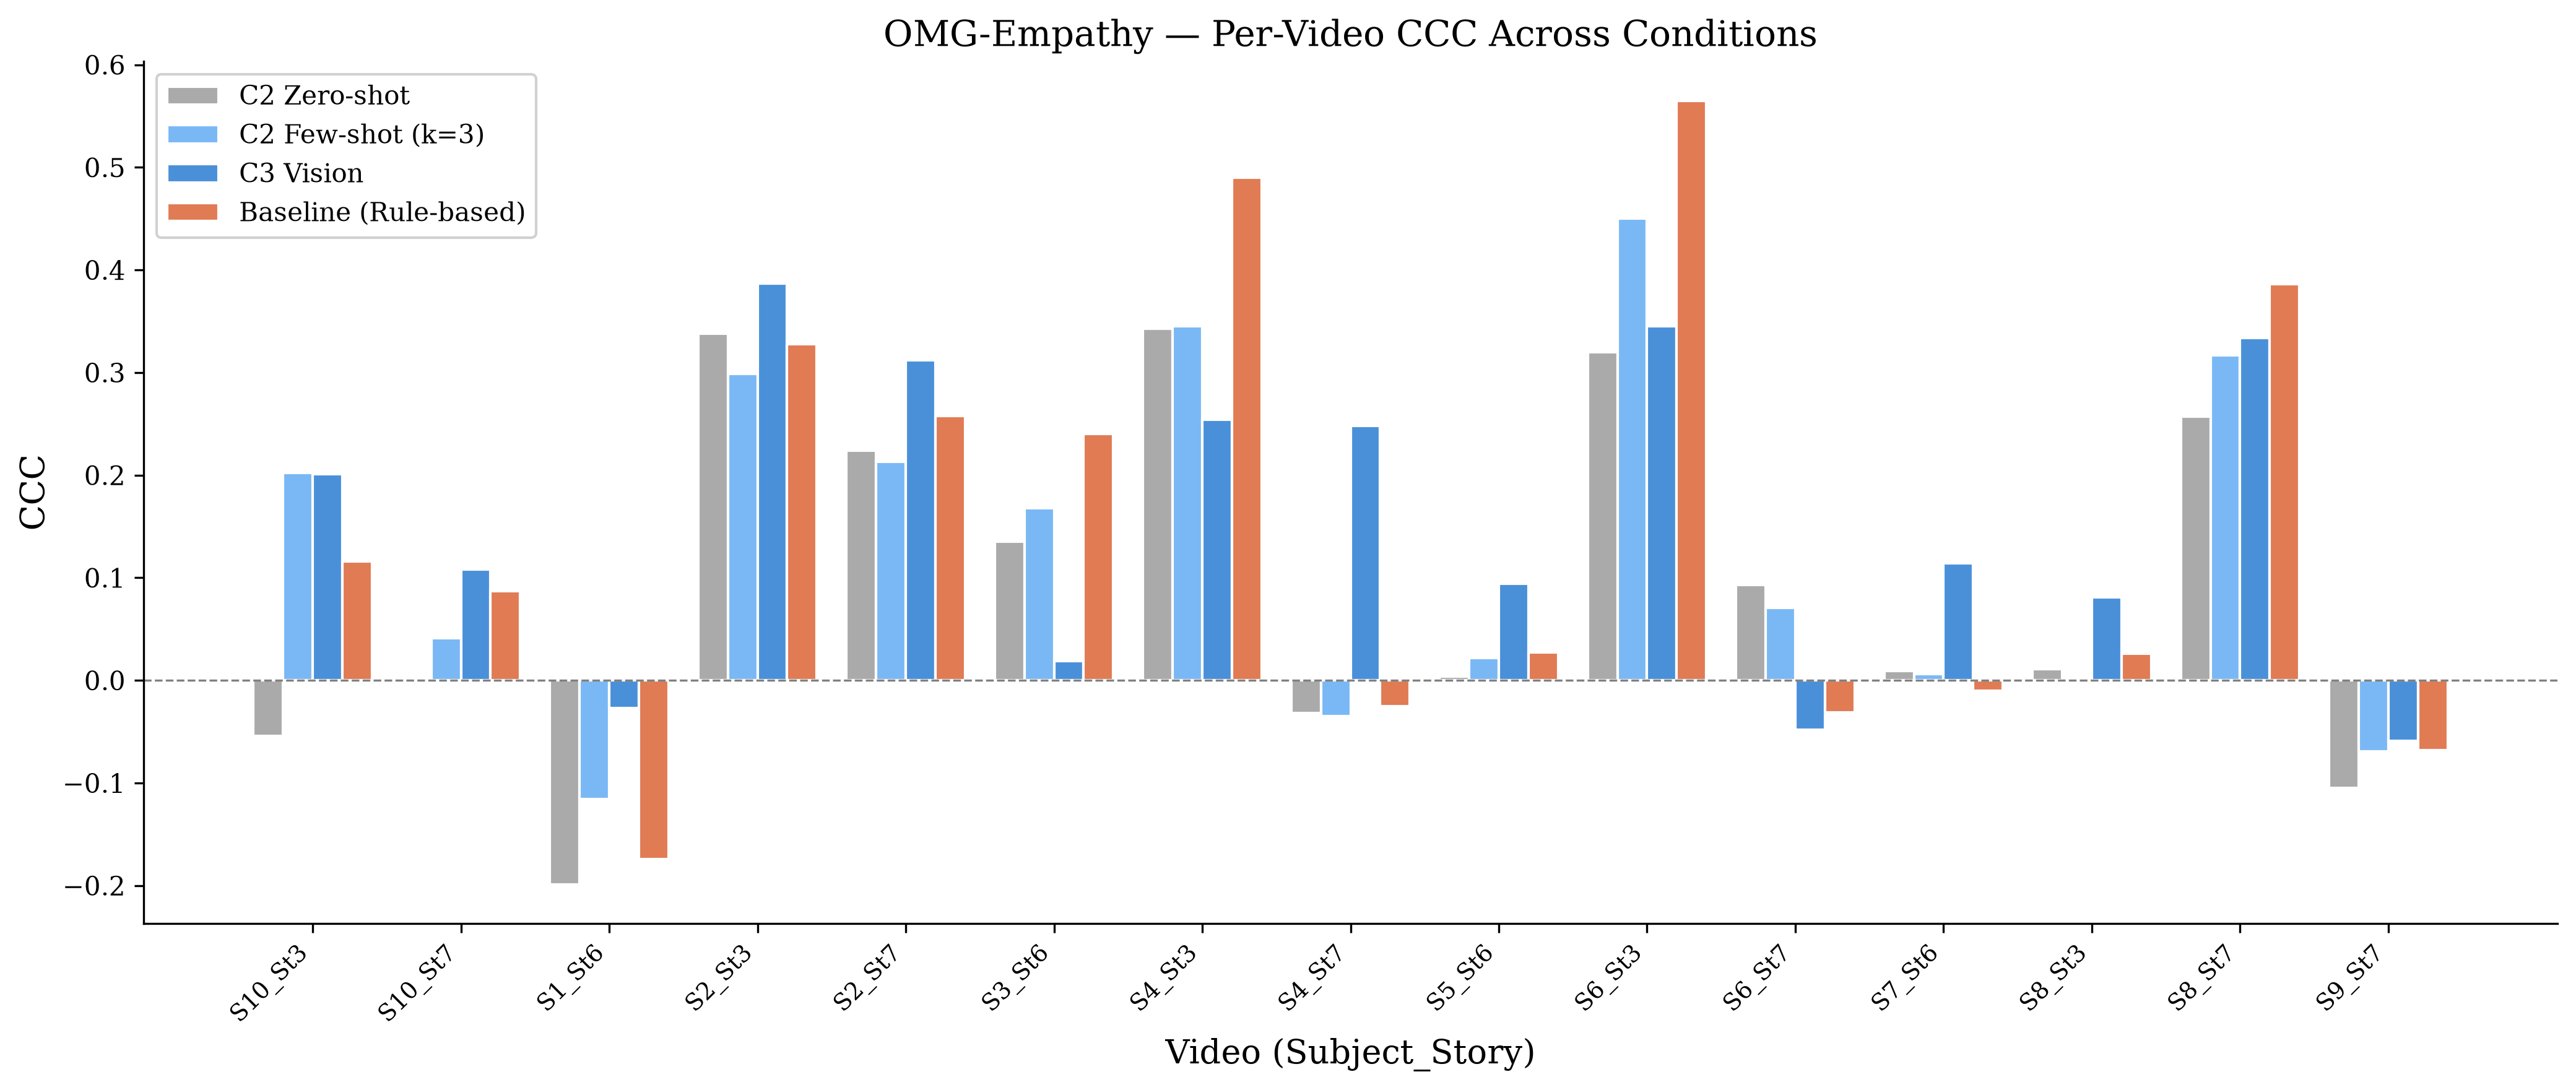
\includegraphics[width=0.92\textwidth]{omg_ccc_per_video.png}
\caption{Per-video CCC across the four systems on OMG-Empathy. Performance varies widely across subjects and stories (SD between 0.15 and 0.21), with subjects 2 and 6 (story 3) consistently easiest and subjects 1 and 9 yielding negative CCC for every method.}
\label{fig:omg_per_video}
\end{figure*}

\subsection{CMU-MOSEI: Multi-Label Emotion Classification}
Table~\ref{tab:mosei_f1} compares all systems on the 400 test segments, and Figure~\ref{fig:mosei_conditions} plots the three F1 variants. The text-based model (C1) reaches a macro-F1 of 0.416, ahead of the trained logistic-regression baseline at 0.333, an improvement of roughly 25\%. The advantage holds across micro-F1 (0.499 vs.\ 0.376) and weighted-F1 (0.498 vs.\ 0.423), and few-shot examples add little (a gain of 0.017 in micro-F1), which suggests that the model already carries the relevant emotional semantics from pre-training.

\begin{table}[htbp]
\caption{Multi-label F1-scores on CMU-MOSEI (400 test segments).}
\label{tab:mosei_f1}
\centering
\setlength{\tabcolsep}{4pt}
\renewcommand{\arraystretch}{1.15}
\small
\begin{tabular}{l c c c}
\hline
\textbf{System} & \textbf{Micro} & \textbf{Macro} & \textbf{Weighted} \\
\hline
Random chance & 0.313 & --- & --- \\
Majority (\emph{happiness}) & 0.391 & 0.108 & 0.214 \\
Baseline (LogReg on FACET) & 0.376 & 0.333 & 0.423 \\
LLM C1 (text), 0-shot & 0.482 & \textbf{0.416} & 0.493 \\
LLM C1 (text), $k=5$ & \textbf{0.499} & \textbf{0.416} & 0.498 \\
LLM C2 (FACET), 0-shot & 0.111 & 0.057 & 0.096 \\
LLM C2 (FACET), $k=5$ & 0.289 & 0.130 & 0.213 \\
\hline
\end{tabular}
\end{table}

\begin{figure}[!ht]
\centering
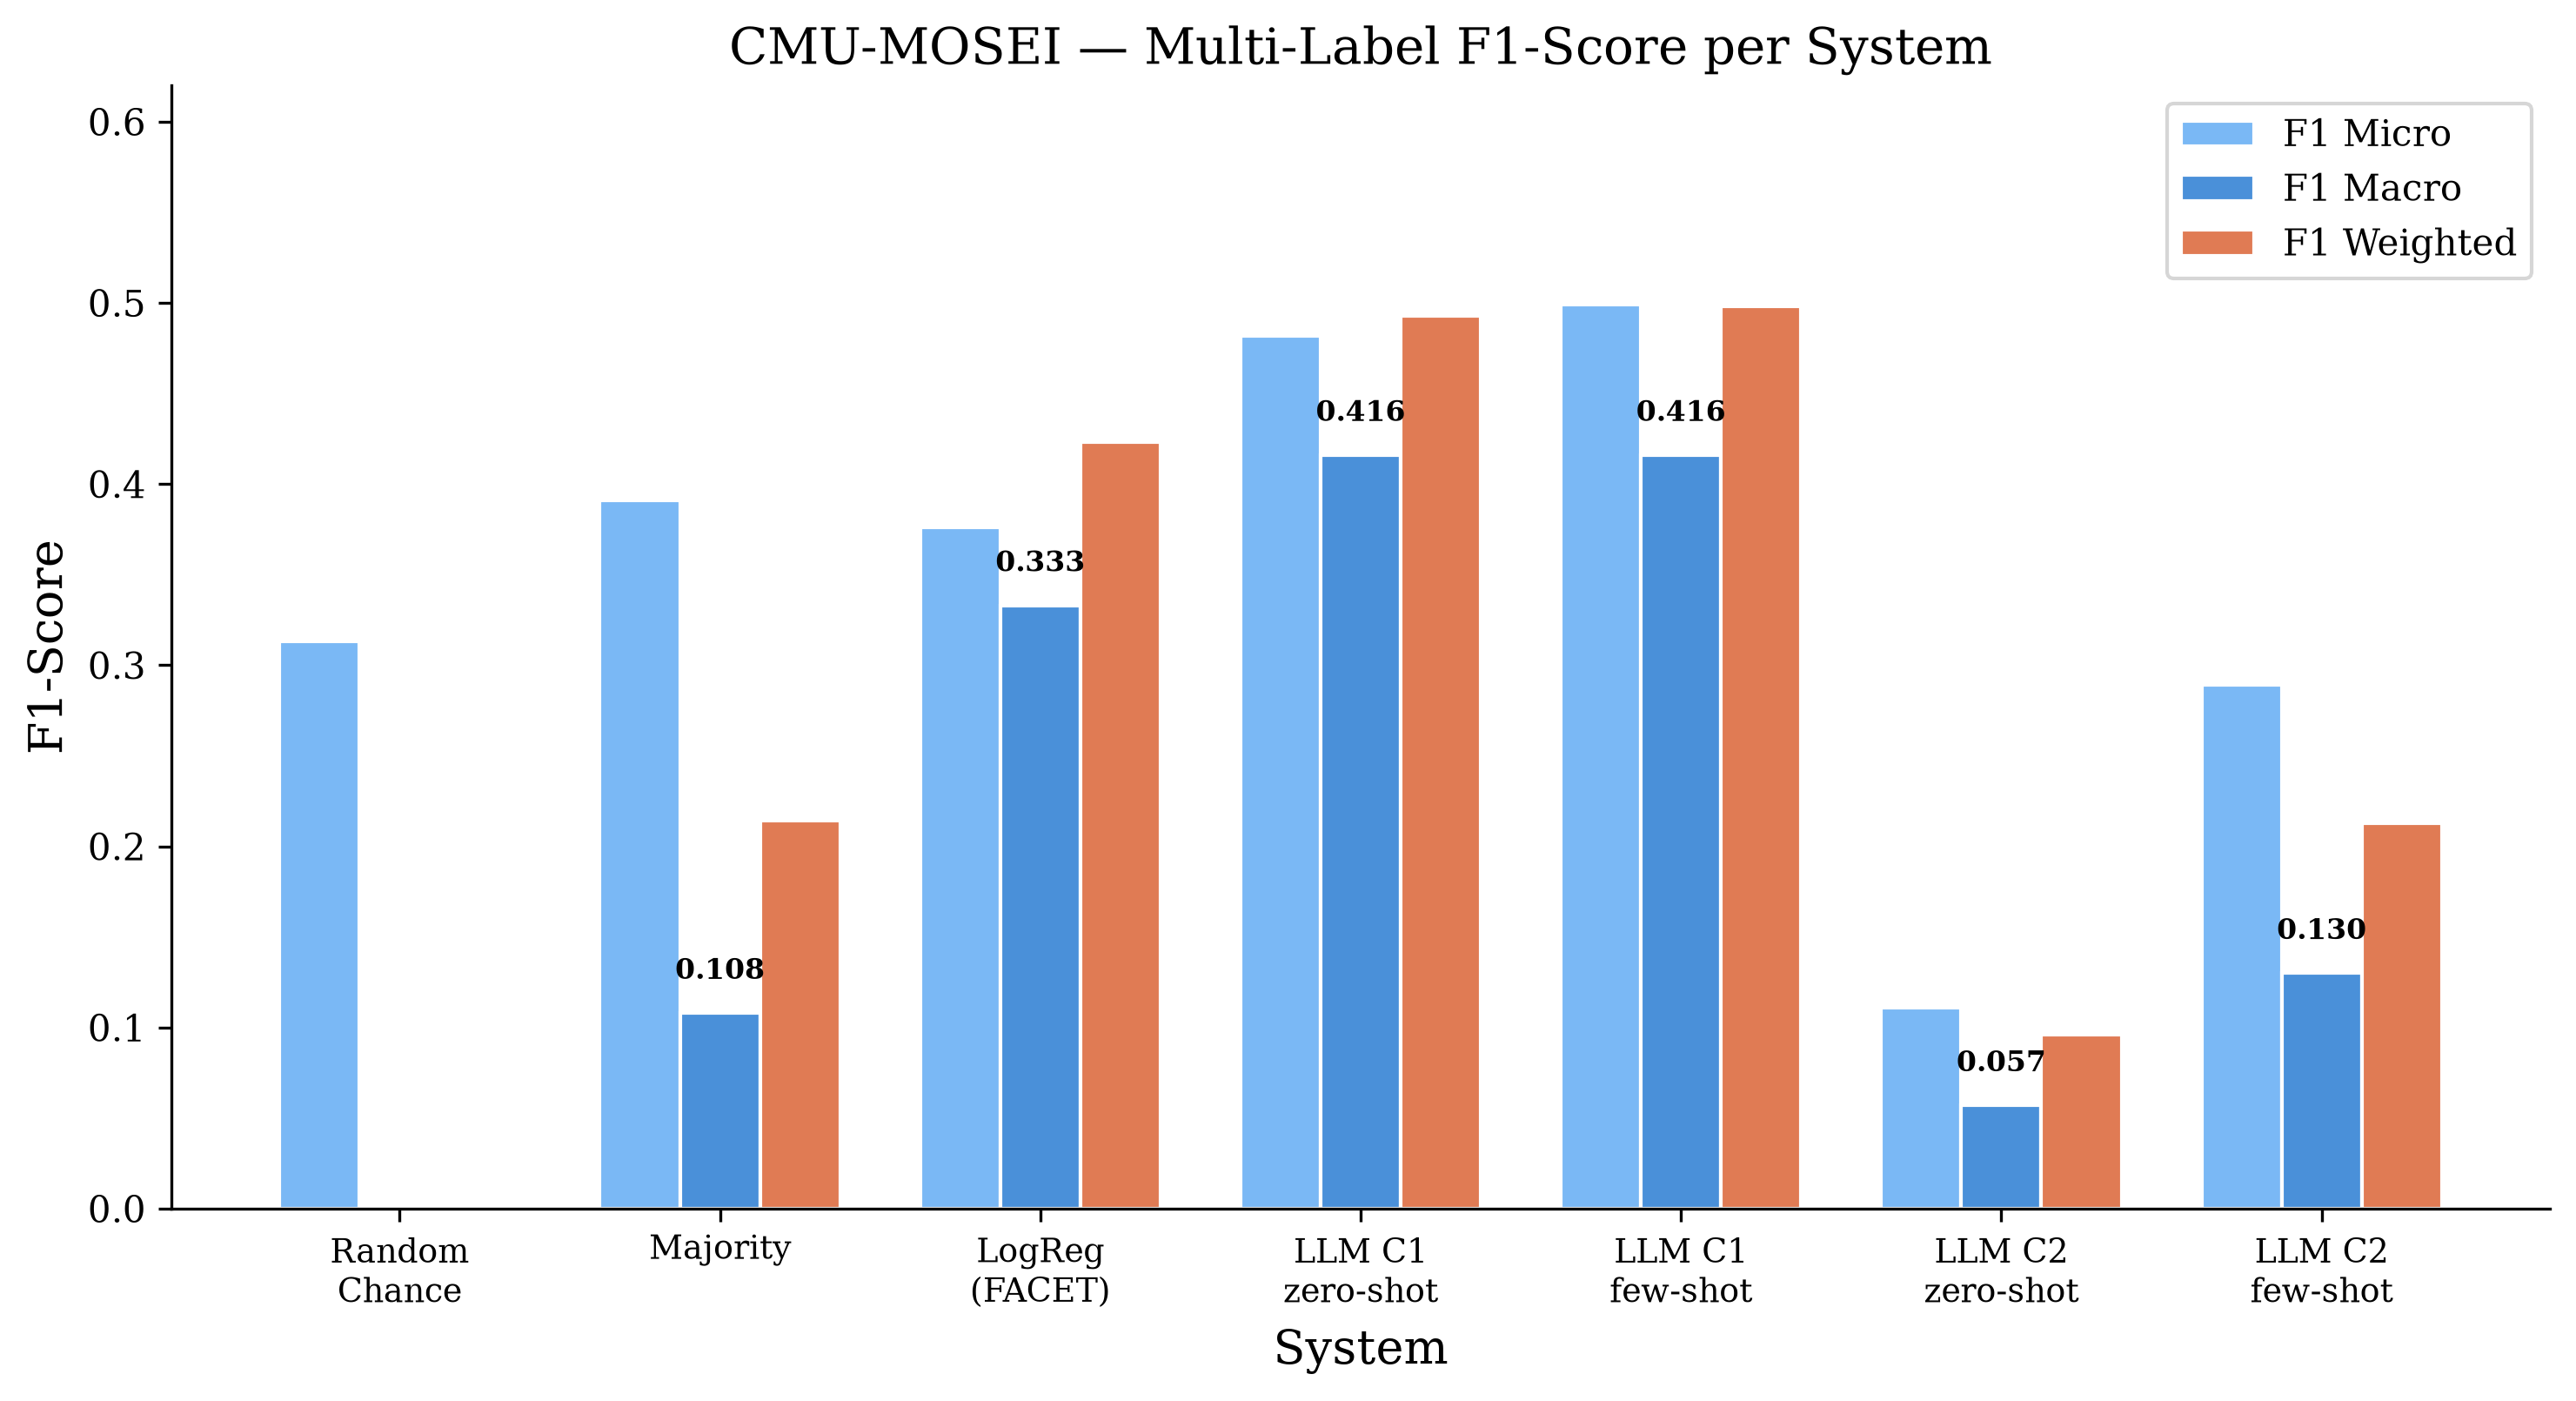
\includegraphics[width=0.46\textwidth]{mosei_f1_conditions.png}
\caption{Multi-label F1 (micro, macro, weighted) for all systems on CMU-MOSEI. The text conditions (C1) lead, while the FACET-based condition (C2) falls below random chance in the zero-shot setting.}
\label{fig:mosei_conditions}
\end{figure}

The contrast with structured features is stark. Given raw FACET vectors (C2), the model collapses to a macro-F1 of 0.057 in zero-shot, below random chance on micro-F1. Few-shot examples recover part of this ($0.057 \rightarrow 0.130$, a $2.3\times$ gain) but leave it far behind the trained baseline. This mirrors the OMG pattern: serialized numerical features are the representation the model cannot use.

\subsection{Per-Emotion Analysis}
Table~\ref{tab:mosei_emotion} and Figure~\ref{fig:mosei_emotion} break the F1 down by Ekman category. The text-based model beats the baseline in five of six categories, with its largest gains on \emph{anger} ($+0.27$) and \emph{disgust} ($+0.14$), precisely the classes where a FACET classifier suffers from imbalance and limited discriminative power. Bootstrap 95\% confidence intervals (10{,}000 resamples) confirm that the gains on anger ($[+0.18, +0.35]$) and disgust ($[+0.06, +0.22]$) are statistically reliable, as both intervals exclude zero. Conversely, the LLM's deficit on happiness ($[-0.10, +0.03]$) and its advantage on the remaining categories (sadness, fear, surprise) have intervals that include zero. The baseline keeps a narrow edge only on \emph{happiness} (0.60 vs.\ 0.57), the dominant class where frequency-based prediction is naturally strong. This is consistent with the view that LLMs hold strong linguistic priors for emotion~\cite{Survey2024AffectiveLLM}, though as Zhang et al.~\cite{Zhang2025FluentUnfeeling} caution, theory-consistent labels do not always reflect fine contextual cues, a subtlety our category-level macro-F1 does not penalize.

\begin{table}[htbp]
\caption{Per-emotion F1: LLM text (C1) vs.\ FACET baseline. $\Delta$ is the best LLM minus the baseline.}
\label{tab:mosei_emotion}
\centering
\setlength{\tabcolsep}{4pt}
\renewcommand{\arraystretch}{1.15}
\small
\begin{tabular}{l c c c c c}
\hline
\textbf{Emotion} & \textbf{Prev.} & \textbf{Base.} & \textbf{C1 0-shot} & \textbf{C1 $k{=}5$} & \boldmath$\Delta$ \\
\hline
happiness & 0.42 & \textbf{0.60} & 0.56 & 0.57 & $-0.03$ \\
sadness & 0.31 & 0.37 & \textbf{0.40} & 0.38 & +0.03 \\
anger & 0.32 & 0.25 & 0.48 & \textbf{0.52} & \textbf{+0.27} \\
fear & 0.04 & 0.07 & \textbf{0.16} & 0.14 & +0.09 \\
disgust & 0.30 & 0.49 & \textbf{0.63} & \textbf{0.63} & \textbf{+0.14} \\
surprise & 0.12 & 0.21 & \textbf{0.26} & 0.25 & +0.05 \\
\hline
\end{tabular}
\end{table}

\begin{figure}[!ht]
\centering
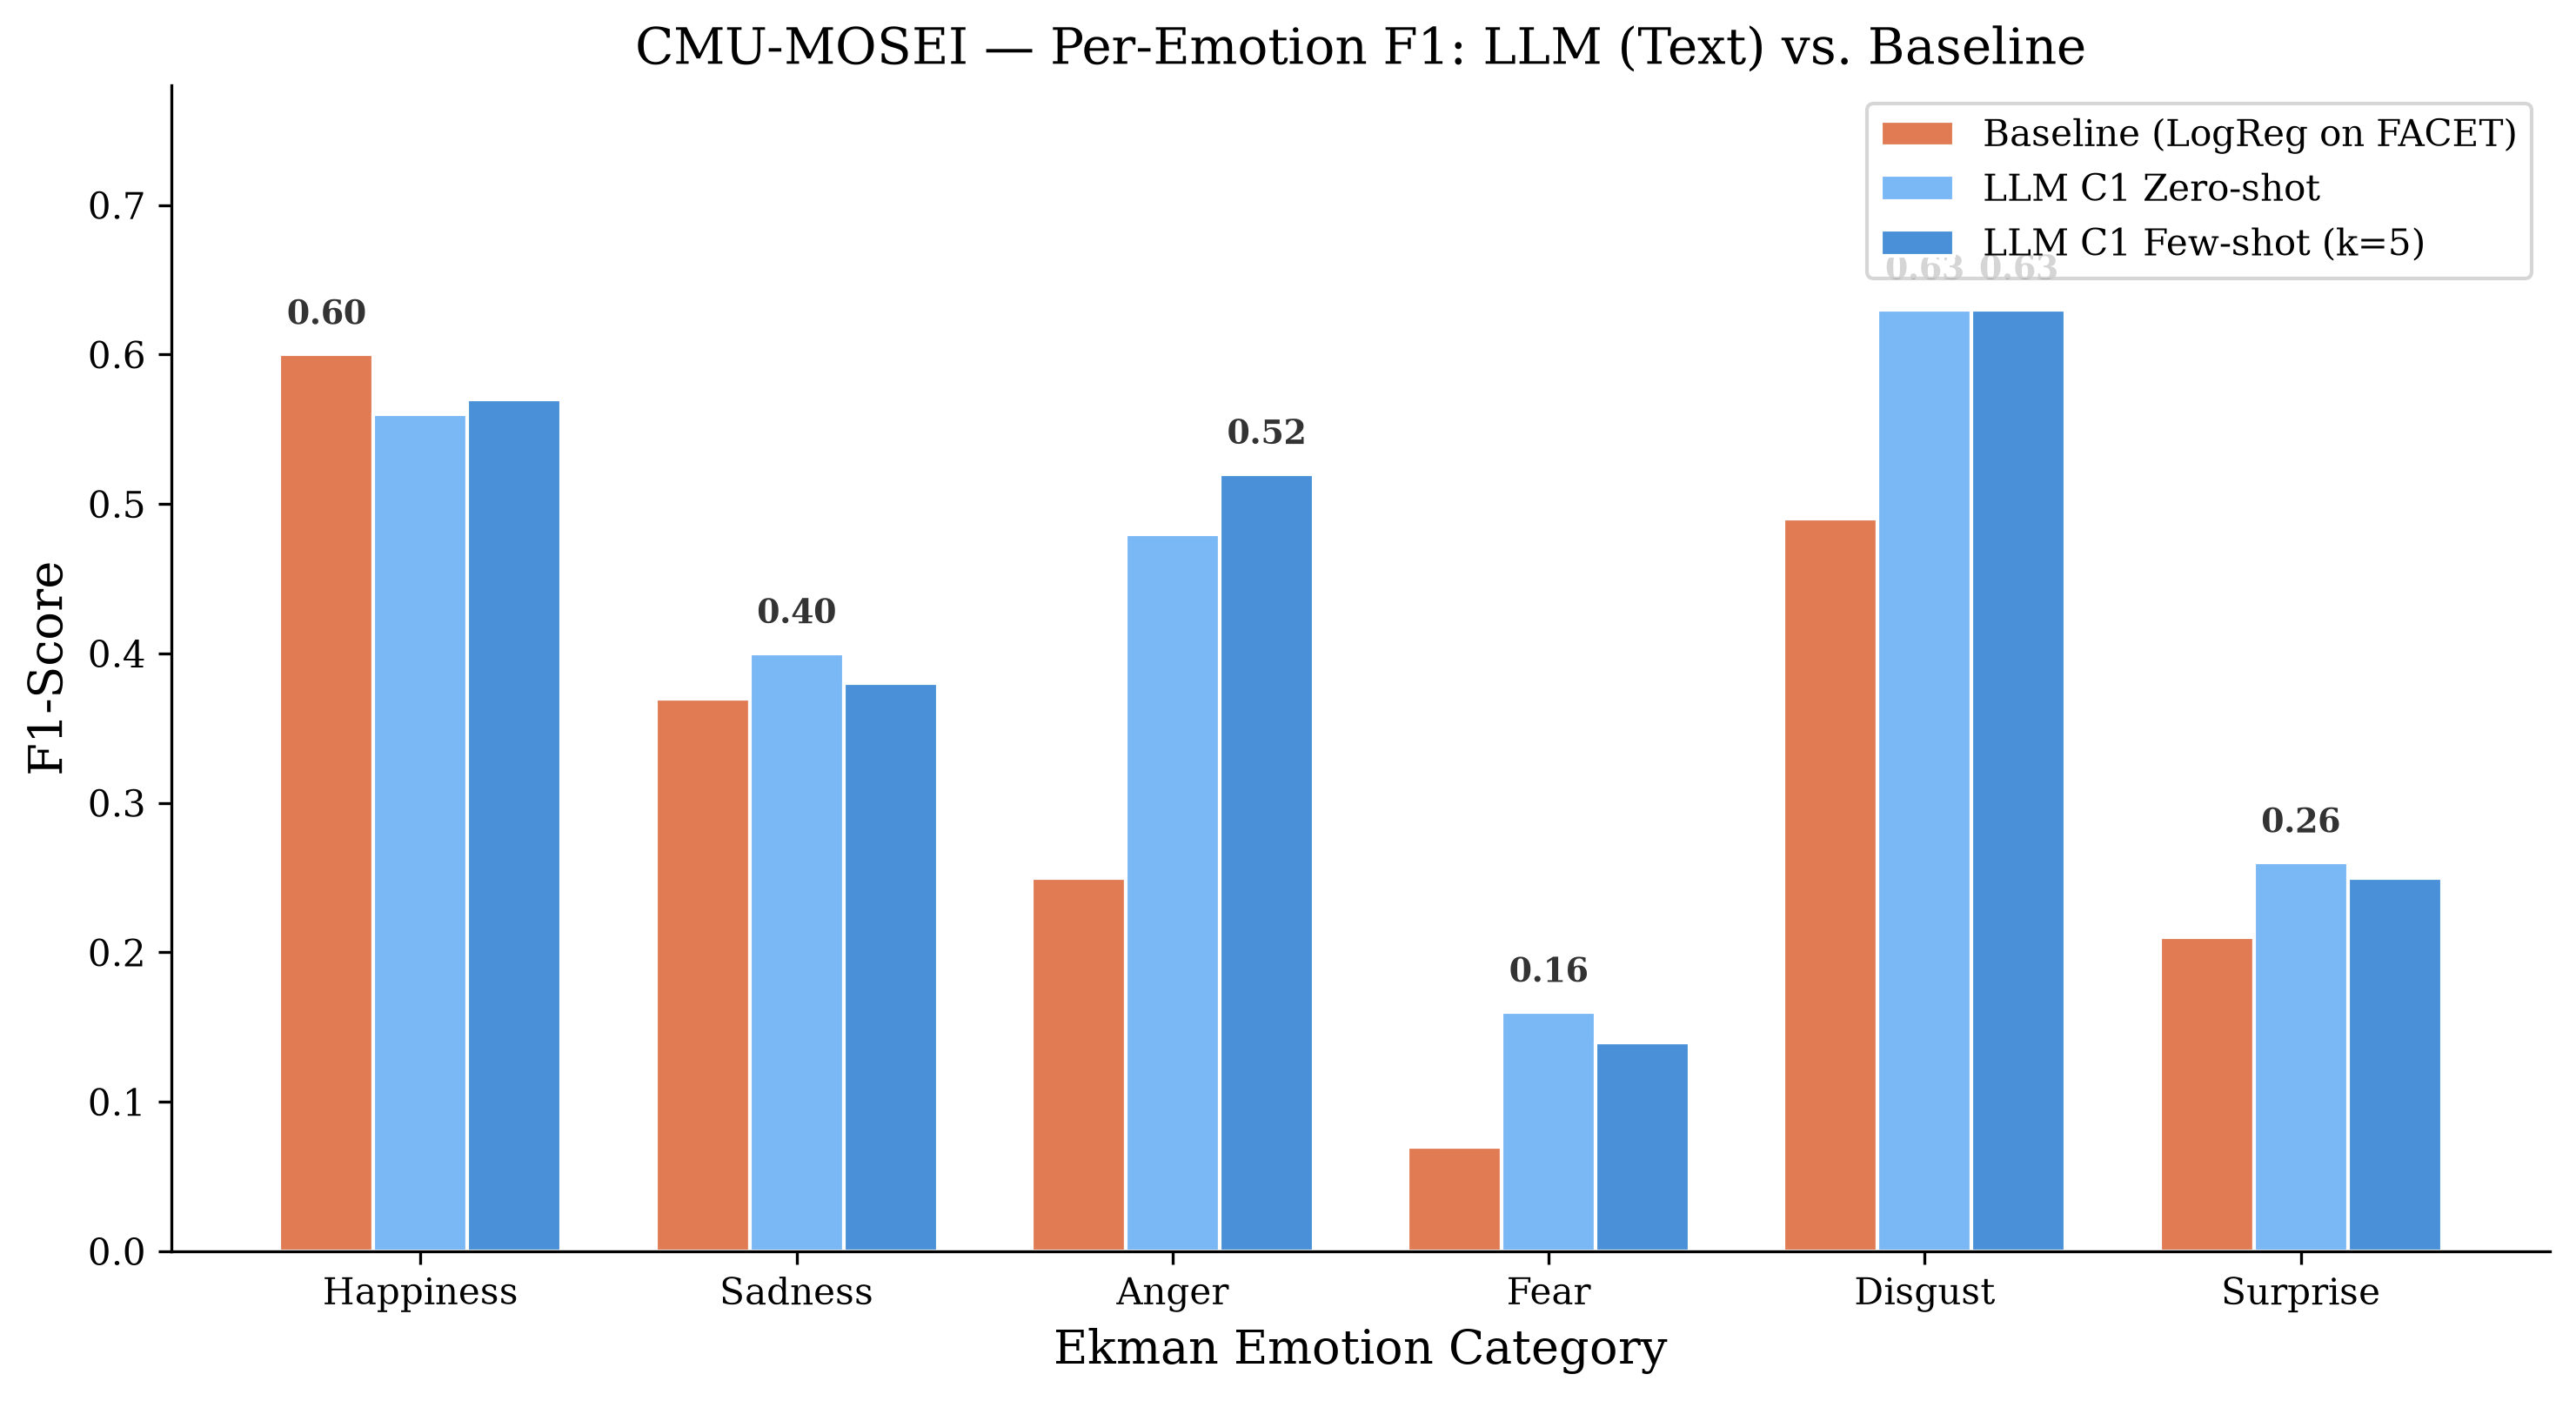
\includegraphics[width=0.46\textwidth]{mosei_f1_per_emotion.png}
\caption{Per-emotion F1 comparison on CMU-MOSEI. The largest LLM gains appear on minority emotions (anger, disgust); the baseline retains a small advantage on the majority class (happiness).}
\label{fig:mosei_emotion}
\end{figure}

\subsection{Statistical Significance of the Text--Feature Gap}
To quantify the gap between the two LLM representations on MOSEI, we computed per-sample F1 (paired, $n=400$) and applied non-parametric tests~\cite{Wilcoxon1945, Cohen1988, Efron1993Bootstrap}, summarized in Table~\ref{tab:mosei_stats}. The mean per-sample F1 is $0.460 \pm 0.429$ for text and $0.329 \pm 0.429$ for FACET, a difference of $+0.131$ whose bootstrap 95\% interval $[+0.079, +0.185]$ excludes zero. The Wilcoxon test is highly significant ($p<0.001$), although the effect size is small ($d=0.24$) owing to high inter-sample variance. A McNemar test on exact label-set match does not reach significance ($p=0.086$), which indicates that the advantage of text appears in partial matches rather than in all-or-nothing correctness. The confidence intervals for the two conditions do not overlap (text $[0.418, 0.502]$, FACET $[0.287, 0.371]$), confirming that the gap is systematic rather than driven by outliers.

To test whether the gap extends to an omnibus comparison across multiple systems, we computed per-sample F1 for deterministic baselines (random chance with class-proportional sampling and majority predicting \emph{happiness}) alongside the two LLM conditions. A Kruskal--Wallis test~\cite{KruskalWallis1952} --- the non-parametric equivalent of a one-way ANOVA, chosen because the per-sample F1 distributions are heavily skewed --- rejects the null hypothesis that all four distributions share the same median ($H=29.18$, $p<10^{-5}$). Dunn~\cite{Dunn1964} post-hoc comparisons with Bonferroni correction show that LLM C1 is significantly better than both LLM C2 ($p<10^{-6}$) and the majority baseline ($p=0.046$), while LLM C2 is significantly worse than random chance ($p=0.001$). The small effect size ($\eta^2 = 0.016$) reflects the high inter-sample variance that is typical of multi-label classification at the individual level.

\begin{table}[htbp]
\caption{Paired statistical tests on MOSEI: C1 (text) vs.\ C2 (FACET), $n=400$.}
\label{tab:mosei_stats}
\centering
\setlength{\tabcolsep}{4pt}
\renewcommand{\arraystretch}{1.15}
\small
\begin{tabular}{l c c}
\hline
\textbf{Test} & \textbf{Statistic} & \textbf{p-value} \\
\hline
Wilcoxon signed-rank (per-sample F1) & $W=7049$ & \textbf{$<0.001$} \\
McNemar (exact set match) & $\chi^2=2.94$ & 0.086 \\
Cohen's $d$ (paired F1) & $+0.243$ & --- \\
Bootstrap 95\% CI ($\Delta$ mean F1) & [+0.079, +0.185] & --- \\
\hline
\end{tabular}
\end{table}

\section{Discussion}
\label{sec:discussion}
The results answer the research question directly: the LLM's advantage over traditional methods is not general but depends on how affective information is represented. Table~\ref{tab:summary} consolidates the picture across both tasks.

\begin{table}[htbp]
\caption{Comparative advantage by modality and task.}
\label{tab:summary}
\centering
\setlength{\tabcolsep}{4pt}
\renewcommand{\arraystretch}{1.15}
\small
\begin{tabular}{p{3.4cm} l p{2.4cm}}
\hline
\textbf{Modality / task} & \textbf{Winner} & \textbf{Evidence} \\
\hline
Emotion from text (MOSEI, C1) & LLM & macro-F1 +25\%; $p<0.001$ \\
Valence from vision (OMG, C3) & Tie & $p=0.421$; rank 1.87 \\
Valence from features (OMG, C2, $k{=}3$) & Slight tie & $p=0.229$ \\
Valence from features (OMG, C2, 0-shot) & Traditional & $p=0.013$ \\
Emotion from FACET (MOSEI, C2) & Traditional & $p<0.001$ \\
\hline
\end{tabular}
\end{table}

\textbf{Text plays to the model's strength.} When the signal is language, the LLM draws on its pre-training to recognize emotional content with zero-shot accuracy that exceeds a classifier trained on thousands of labeled examples. This is the clearest and most significant result in the study, and it aligns with the broader trend reported in recent surveys~\cite{Survey2024AffectiveLLM, Survey2025MLLMEmotion}.

\textbf{Vision is competitive.} Reading raw keyframes, the model matches the rule-based blendshape engine on continuous valence ($p=0.421$) and ranks first under the Friedman analysis. Neither method achieves high absolute CCC, but the model does so without any feature engineering, processing pixels end to end. This suggests that native vision is a viable route for facial affect even if it is not yet decisively better than a tuned rule set.

\textbf{Structured features defeat the model.} When facial information is serialized as numbers, performance collapses: below the trained baseline on OMG ($p=0.013$) and below random chance on MOSEI. The bottleneck is representational. A tokenizer splits multi-digit values into pieces, and the magnitude relations that a logistic regression reads directly from a vector are simply not available to the model in this form~\cite{Survey2024TextCentric}. Few-shot examples help (Table~\ref{tab:fewshot}) but do not close the gap, which confirms that the problem is the encoding rather than the task framing.

\begin{table}[htbp]
\caption{Effect of few-shot learning across conditions.}
\label{tab:fewshot}
\centering
\setlength{\tabcolsep}{4pt}
\renewcommand{\arraystretch}{1.15}
\small
\begin{tabular}{l c c c}
\hline
\textbf{Condition} & \textbf{Zero-shot} & \textbf{Few-shot} & \textbf{Change} \\
\hline
C1 text (MOSEI, macro-F1) & 0.416 & 0.416 & +0\% \\
C2 blendshapes (OMG, CCC) & +0.090 & +0.127 & +41\% \\
C2 FACET (MOSEI, macro-F1) & 0.057 & 0.130 & +128\% \\
\hline
\end{tabular}
\end{table}

\textbf{Implications for social robotics.} These findings speak directly to how affective perception should be organized in a cognitive architecture for HRI~\cite{Goodrich2007HRISurvey, Breazeal2003SociableRobots}. Rule-based and traditional pipelines that operate on structured facial descriptors remain competitive for real-time, feature-level perception, which is the regime targeted by blendshape-based affective systems for robots~\cite{Spitale2024AffectiveRobotics}. An LLM is the wrong tool to hand a stream of numbers, but the right tool to interpret what a partner said, where it captures nuanced states such as anger, disgust, and fear that feature-based classifiers miss. Work on LLM-driven social robots points in the same direction, integrating affective reasoning with language to improve perceived empathy~\cite{Magalhaes2024Nadine, Churamani2024EmpathicGrounding}. Taken together, the evidence favors a hybrid architecture: lightweight feature-based perception for the real-time loop, and an LLM as a higher-level affective reasoner over text and raw imagery where latency budgets allow. This division of labor mirrors how LLMs are already used as reasoning cores rather than low-level controllers in robotics~\cite{Ahn2022SayCan, Zitkovich2023RT2, Kawaharazuka2024RobotLLMSurvey}.

\section{Computational Cost and Inference Time}
\label{sec:cost}
Any robotic deployment must weigh accuracy against cost, an aspect frequently raised by reviewers and practitioners alike. Table~\ref{tab:model} summarizes the model and serving configuration, Table~\ref{tab:latency} reports per-condition token budgets and measured latencies, and Figure~\ref{fig:latency} shows the latency distributions.

\begin{table}[htbp]
\caption{Model architecture and serving configuration.}
\label{tab:model}
\centering
\setlength{\tabcolsep}{4pt}
\renewcommand{\arraystretch}{1.15}
\small
\begin{tabular}{l l}
\hline
\textbf{Parameter} & \textbf{Value} \\
\hline
Model & Gemma 4 26B-A4B-it (AWQ 4-bit) \\
Architecture & MoE: 25.2\,B total, 3.8\,B active \\
Layers / experts & 30 layers, 128 experts (top-8 + 1) \\
Vision encoder & SigLIP ($\sim$550\,M, frozen) \\
Context window & 262{,}144 tokens \\
Memory footprint & $\sim$13.5\,GB \\
Serving engine & vLLM (PagedAttention) \\
Hardware & NVIDIA L4 24\,GB (GCP Spot VM) \\
Decoding & Greedy ($T=0$), max 512 tokens \\
\hline
\end{tabular}
\end{table}

\begin{table}[htbp]
\caption{Estimated token budget and measured latency per condition.}
\label{tab:latency}
\centering
\setlength{\tabcolsep}{3pt}
\renewcommand{\arraystretch}{1.15}
\footnotesize
\begin{tabular}{l c c c c c}
\hline
\textbf{Condition} & \textbf{Tokens} & \textbf{Median} & \textbf{Mean} & \textbf{P95} & \textbf{N} \\
\hline
OMG C2 (0-shot) & $\sim$570 & 918\,ms & 1035\,ms & 1609\,ms & 240 \\
OMG C3 (0-shot) & $\sim$3850 & 2387\,ms & 4553\,ms & 15635\,ms & 240 \\
MOSEI C1 (0-shot) & $\sim$390 & 1817\,ms & 1828\,ms & 1923\,ms & 400 \\
MOSEI C2 (0-shot) & $\sim$590 & 1860\,ms & 1872\,ms & 1954\,ms & 400 \\
\hline
\end{tabular}
\end{table}

\begin{figure}[!ht]
\centering
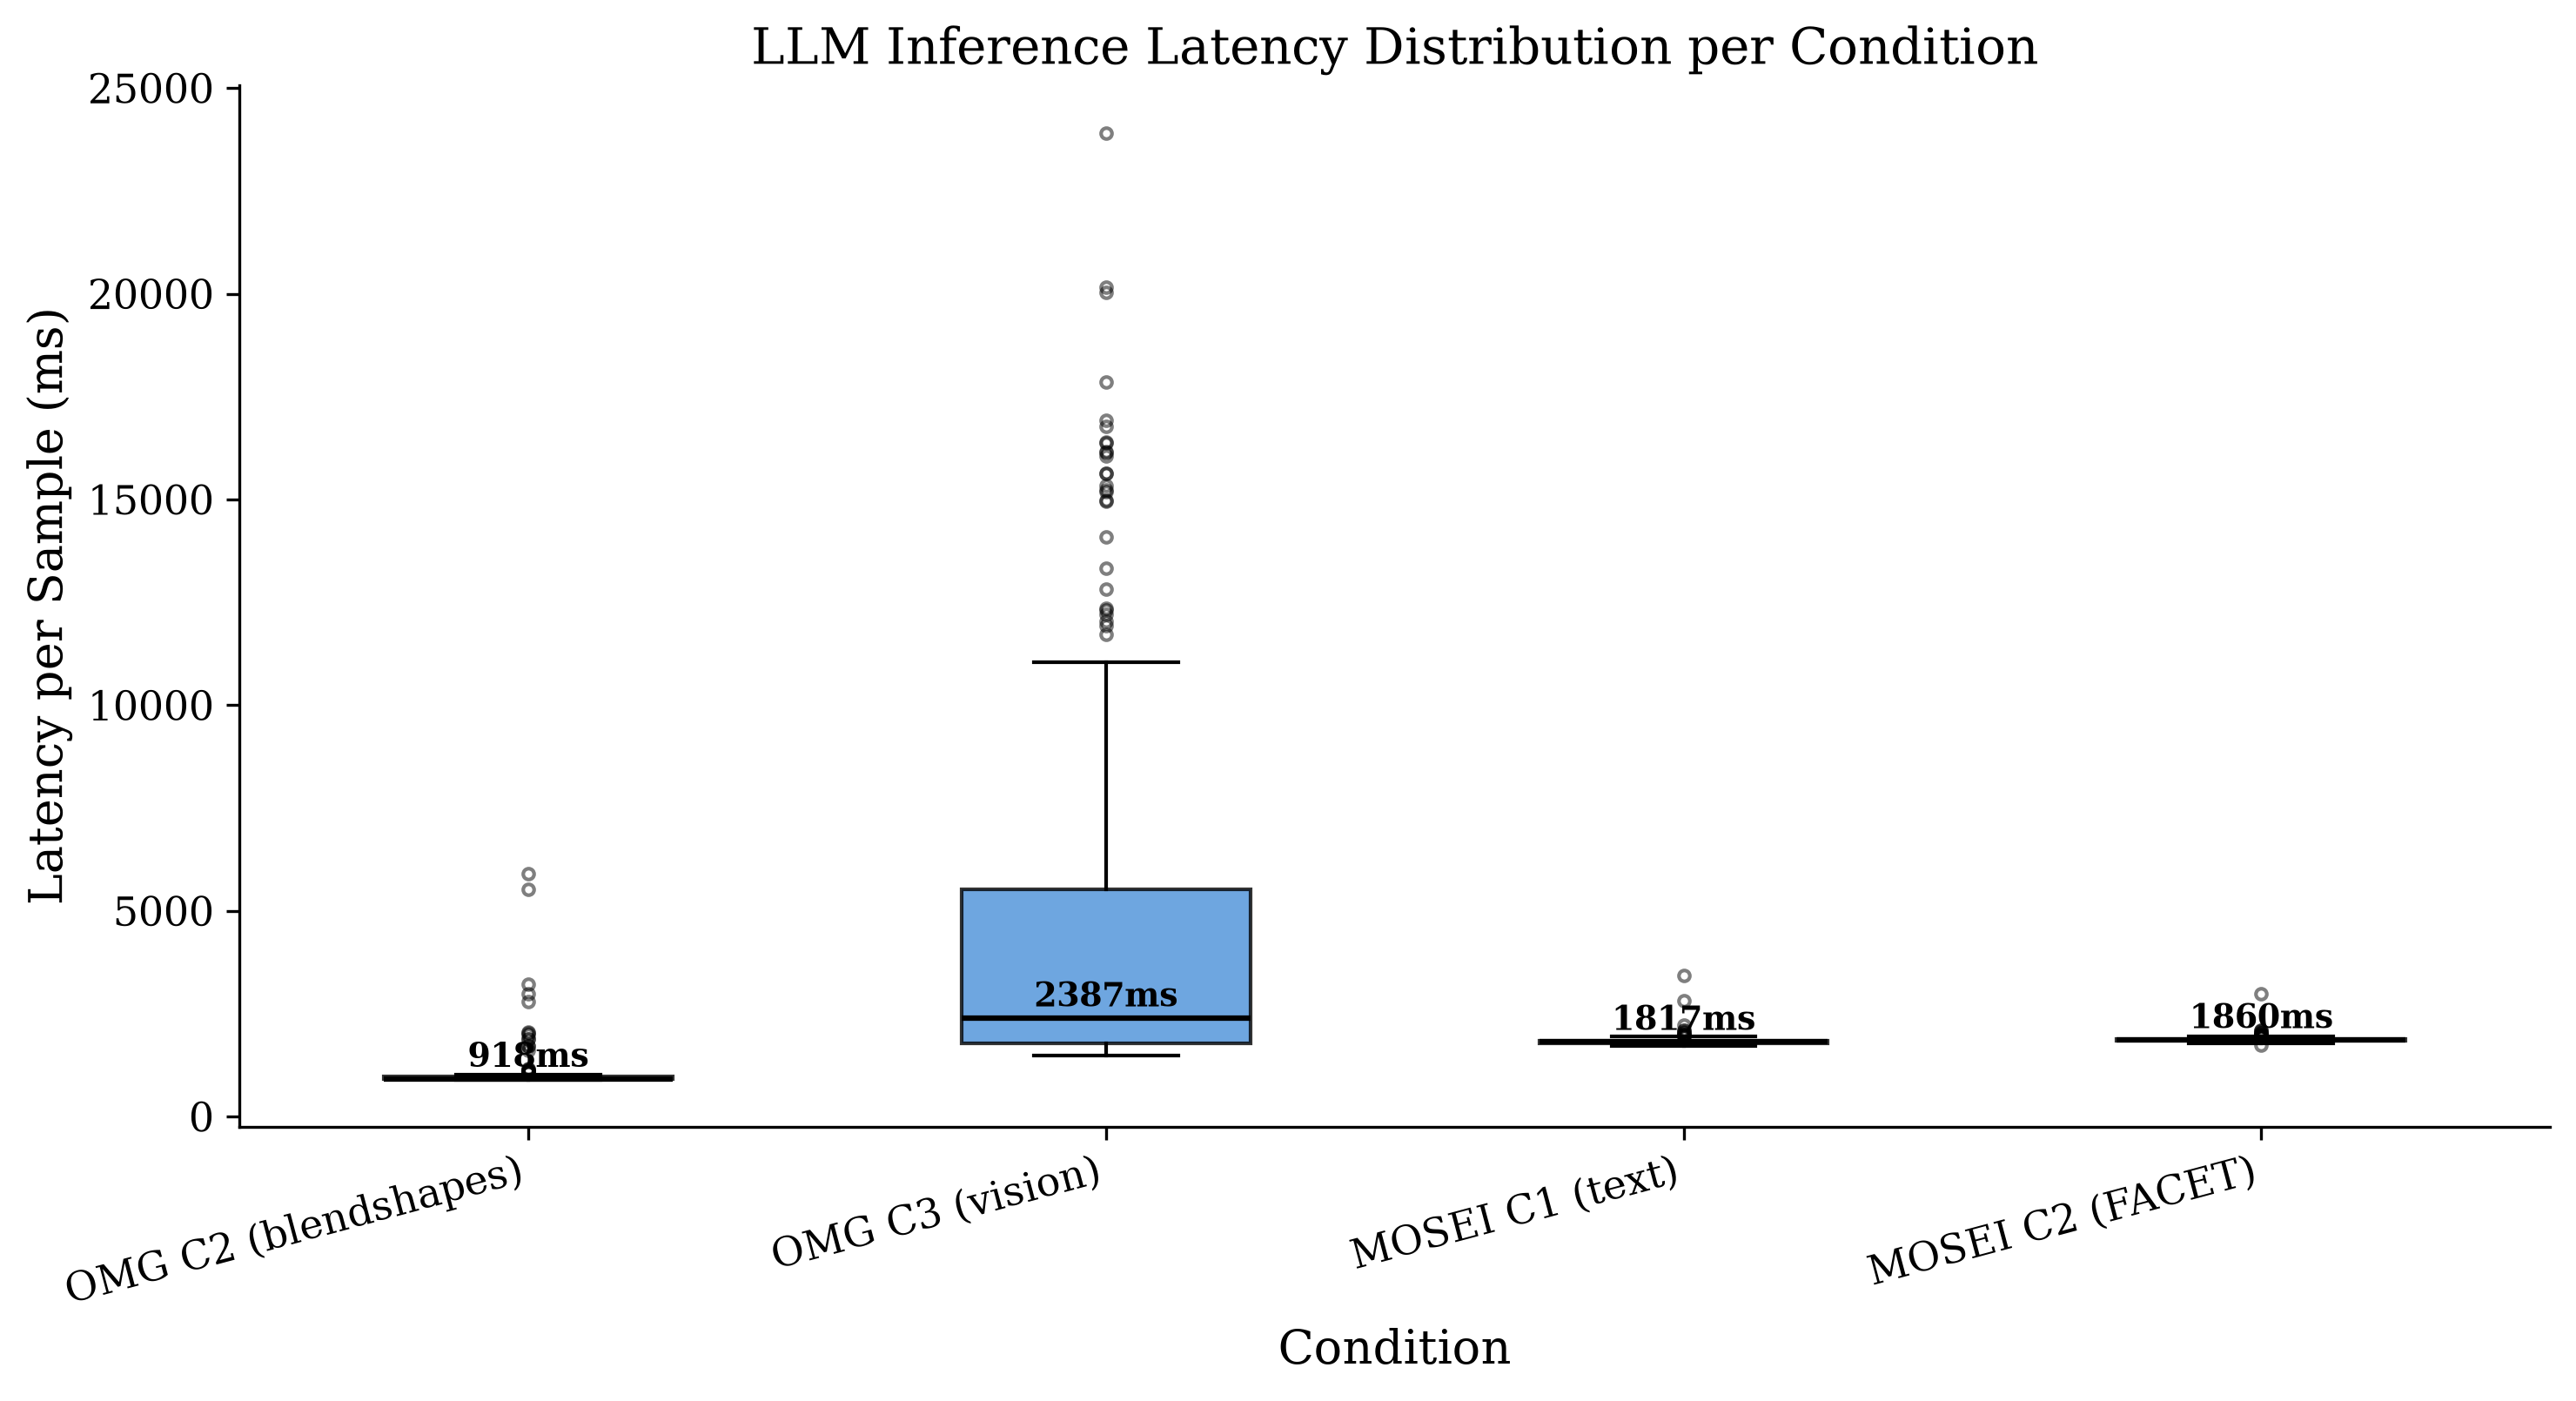
\includegraphics[width=0.46\textwidth]{latency_boxplot.png}
\caption{Per-sample inference latency by condition. The vision condition (C3) is both slower and far more variable than the text and feature conditions, reflecting the cost of encoding three keyframes through the vision encoder.}
\label{fig:latency}
\end{figure}

The vision condition is about $4.4\times$ slower than the text-only conditions because each window encodes three JPEG keyframes (roughly 1{,}200 visual tokens per image). Text and feature conditions show low and stable latency (standard deviation between 74 and 113\,ms), whereas vision is heavy-tailed, with a 95th percentile near 15.6\,s. A Kruskal--Wallis test~\cite{KruskalWallis1952} confirms that all four conditions differ significantly in latency ($H=621.96$, $p<10^{-134}$, $\eta^2 \approx 0.49$), and Dunn~\cite{Dunn1964} post-hoc comparisons with Bonferroni correction show that every pairwise difference is significant ($p<0.05$ in all six pairs), including the relatively close MOSEI C1 versus C2 ($p<10^{-15}$). Across all 1{,}280 inference calls the campaign used about 47 minutes of GPU time, or roughly \$0.19 at the spot price of an L4, which makes evaluation at this scale inexpensive even with a 26\,B-parameter model.

The trade-off against the baselines is, however, severe. As shown in Table~\ref{tab:tradeoff}, the LLM requires a GPU and runs three orders of magnitude slower than a rule engine or a logistic regression. At one to five seconds per sample it is unsuitable for frame-level perception at 30\,fps, but it remains usable at the interaction-turn level, for example when analyzing a four-second dialogue window, and could be accelerated through batching, speculative decoding~\cite{Kwon2023vLLM}, or smaller distilled models.

\begin{table}[htbp]
\caption{Computational requirements: LLM vs.\ traditional baselines.}
\label{tab:tradeoff}
\centering
\setlength{\tabcolsep}{4pt}
\renewcommand{\arraystretch}{1.15}
\small
\begin{tabular}{l l l}
\hline
\textbf{Metric} & \textbf{LLM} & \textbf{Baseline} \\
\hline
GPU required & Yes (L4 24\,GB) & No (CPU) \\
Model memory & $\sim$13.5\,GB & $<$1\,MB \\
Active params & 3.8\,B & $<$1\,K \\
Latency (text C1) & $\sim$1828\,ms & $<$1\,ms \\
Latency (vision C3) & $\sim$4553\,ms & $\sim$15\,ms \\
Latency (features C2) & $\sim$1035\,ms & $<$1\,ms \\
Real-time (30\,fps) & No & Yes \\
\hline
\end{tabular}
\end{table}

\section{Limitations}
\label{sec:limitations}
Several caveats temper these results. First, we evaluated 15 of the 30 OMG test videos; inter-video variance is high and the full set would increase statistical power. Second, the MOSEI emotion threshold was tuned on the test set itself, which may introduce mild optimistic bias; a held-out validation set should be used for final calibration. Third, results rest on a single prompt template and deterministic decoding, and prompt sensitivity remains a known concern for LLM evaluation~\cite{Zhang2025FluentUnfeeling}. Fourth, MOSEI transcripts come from public YouTube videos that may overlap with the model's pre-training corpus, which could inflate text performance; we declare this without a quantitative estimate. Fifth, the model was quantized to 4-bit via AWQ~\cite{Lin2024AWQ}, and we did not isolate the effect of quantization on affective accuracy. Finally, the baselines, a rule engine and a logistic regression, are not the supervised state of the art~\cite{Li2022DeepFER}; stronger baselines could narrow the text gap.

\section{Conclusion}
\label{sec:conclusion}
We asked how textual, visual, and structured-feature representations influence the affective perception of a multimodal LLM, holding the model fixed and varying only its input. The answer is that representation, not the model alone, governs performance. The LLM reads emotion from text better than a trained classifier, matches a rule-based engine when it sees raw images, and fails when facial information is serialized as numbers, a pattern confirmed by paired tests, a Friedman analysis, and bootstrap intervals across two datasets. For social robotics this argues against treating the LLM as a universal affective sensor and for a hybrid design in which lightweight feature-based components serve the real-time loop while the LLM reasons over language and imagery. Future work includes the full OMG test set, multimodal fusion of text and vision within a single prompt, stronger learned baselines, and integration of the affective module into a closed robot interaction loop.

\section*{Acknowledgment}
This study was partially financed by the Coordena\c{c}\~ao de Aperfei\c{c}oamento de Pessoal de N\'ivel Superior --- Brasil (CAPES) --- Finance Code 001, the Funda\c{c}\~ao de Amparo \`a Ci\^encia e Tecnologia do Estado de Pernambuco (FACEPE), and the Conselho Nacional de Desenvolvimento Cient\'ifico e Tecnol\'ogico (CNPq).

\bibliographystyle{IEEEtran}
\bibliography{references}

\end{document}
